% ============================================================
% CHƯƠNG 4: HIỆN THỰC VÀ THỰC NGHIỆM
% ============================================================
\clearpage
\section{Hiện thực và thực nghiệm}
\label{sec:implementation_experiment}

\subsection{Sơ đồ ánh xạ hiện thực}

Hình~\ref{fig:implementation_architecture} liên kết các thành phần đã mô tả ở thiết kế (Chương 3)
với tệp dữ liệu đầu vào, mã nguồn ETL/Dashboard/Mining và cơ sở dữ liệu SQLite trong kho mã.

\begin{figure}[H]
  \centering
  \resizebox{0.98\textwidth}{!}{%
  \begin{tikzpicture}[
    node distance=5mm,
    font=\sffamily\footnotesize,
    >={Latex[length=2.2mm]},
    arr/.style={->, thick, draw=black!55},
    csv/.style={
      rectangle, rounded corners=2.5pt, draw=orange!75!black, line width=0.8pt,
      minimum width=2.15cm, minimum height=0.62cm, align=center, inner sep=2pt,
      font=\scriptsize
    },
    layer/.style={
      rectangle, rounded corners=4pt, draw=blue!40!black, line width=0.9pt,
      align=center, inner sep=6pt, text width=12.8cm
    },
    app/.style={
      rectangle, rounded corners=4pt, draw=teal!45!black, line width=0.85pt,
      align=left, inner sep=6pt, text width=5.85cm, minimum height=2.1cm
    },
    srcbox/.style={
      rectangle, rounded corners=4pt, draw=orange!50!black, line width=0.7pt,
      dashed, inner sep=6pt
    },
  ]
  
  % --- Ba file CSV ---
  \node[csv] (csv_fl) {\textbf{flights.csv}};
  \node[csv, right=4mm of csv_fl] (csv_al) {\textbf{airlines.csv}};
  \node[csv, right=4mm of csv_al] (csv_ap) {\textbf{airports.csv}};
  
  % --- Khung bao + nhãn bên trong ---
  \node[srcbox, fit=(csv_fl)(csv_al)(csv_ap),
        label={[font=\scriptsize\itshape, text=black!60]above:Nguồn dữ liệu thô (Kaggle 2015)}
  ] (srcframe) {};
  
  % --- ETL ---
  \node[layer, below=10mm of srcframe.south] (etl) {%
    \textbf{Tầng ETL (chuẩn hóa \& tích hợp)}\\[2pt]
    {\scriptsize
    Streaming theo chunk (\texttt{CHUNK\_SIZE}) $\rightarrow$
    \texttt{etl/extract.py} $\rightarrow$ \texttt{etl/transform.py} $\rightarrow$ \texttt{etl/load.py};
    điều phối bởi \texttt{pipeline.py}.}%
  };
  
  % --- Ba mũi tên hội tụ vào etl.north ---
  \draw[arr] (csv_fl.south) -- +(0,-3mm) -| (etl.north);
  \draw[arr] (csv_al.south) -- (etl.north);
  \draw[arr] (csv_ap.south) -- +(0,-3mm) -| (etl.north);
  
  % --- Data Warehouse ---
  \node[layer, below=5mm of etl] (dw) {%
    \textbf{Data Warehouse --- SQLite} \texttt{warehouse/airline\_dw.db}\\[2pt]
    {\scriptsize
    \textbf{Star Schema:} bảng sự kiện \texttt{fact\_flights};
    bảng chiều \texttt{dim\_airline}, \texttt{dim\_airport},
    \texttt{dim\_date}, \texttt{dim\_delay\_reason}.}%
  };
  \draw[arr] (etl.south) -- (dw.north);
  
  % --- Hai nhánh tiêu thụ ---
  \node[app, below left=6mm and 2mm of dw.south west, anchor=north west] (dash) {%
    \textbf{Dashboard phân tích (Streamlit)}\\[2pt]
    {\scriptsize
    Thư mục \texttt{dashboard/}: truy vấn SQL trực tiếp lên DW;
    tổng quan KPI, phân tích tuyến đường, thời gian, nguyên nhân delay,
    explorer, dự báo (\texttt{predict\_service}).}%
  };
  
  \node[app, below right=6mm and 2mm of dw.south east, anchor=north east] (mine) {%
    \textbf{Khai phá dữ liệu (Data Mining)}\\[2pt]
    {\scriptsize
    Thư mục \texttt{mining/}: huấn luyện \& so sánh mô hình
    (\texttt{compare\_5\_models.py}, \texttt{run\_models.py});
    lưu artifact \texttt{.pkl};
    báo cáo HTML \texttt{five\_models\_report.html}.}%
  };
  
  \draw[arr] (dw.south) -- ++(0,-3mm) -| (dash.north);
  \draw[arr] (dw.south) -- ++(0,-3mm) -| (mine.north);
  
  % --- Background ---
  \begin{scope}[on background layer]
    \node[
      fill=gray!4, rounded corners=6pt, inner sep=10pt,
      fit=(srcframe)(mine)(dash), draw=gray!25, dashed
    ] {};
  \end{scope}
  
  \end{tikzpicture}%
  }
  \caption{Sơ đồ ánh xạ hiện thực: tệp dữ liệu đầu vào, module ETL, cơ sở dữ liệu
  triển khai và các thư mục mã nguồn tương ứng trong dự án.}
  \label{fig:implementation_architecture}
  \end{figure}



\subsection{Môi trường thực nghiệm}

\begin{table}[H]
\centering
\caption{Cấu hình môi trường thực nghiệm}
\begin{tabular}{|l|l|}
\hline
\textbf{Thành phần} & \textbf{Thông số} \\ \hline
Hệ điều hành   & Windows 10/11 (64-bit) \\ \hline
CPU            & [Điền thông số CPU] \\ \hline
RAM            & [Điền dung lượng RAM] \\ \hline
Storage        & SSD [Dung lượng] \\ \hline
Python         & 3.10+ \\ \hline
pandas         & 2.x \\ \hline
numpy          & 1.x \\ \hline
scikit-learn   & 1.x \\ \hline
xgboost        & 2.x \\ \hline
lightgbm       & 4.x \\ \hline
tensorflow/keras & 2.x (Neural Network) \\ \hline
plotly / dash  & 5.x \\ \hline
SQLite         & 3.x (qua thư viện \texttt{sqlite3}) \\ \hline
\end{tabular}
\label{tab:environment}
\end{table}

% ------------------------------------------------------------
\subsection{Kết quả ETL}

\subsubsection{Luồng dữ liệu CSV thô vào Database}

Quá trình ETL xử lý 3 file CSV đầu vào và tạo ra Data Warehouse SQLite:

% \begin{figure}[H]
%     \centering
%     \includegraphics[width=0.85\textwidth]{img/etl_flow.png}
%     \caption{Luồng dữ liệu từ CSV thô đến Data Warehouse}
%     \label{fig:etl_flow}
% \end{figure}

\begin{table}[H]
\centering
\caption{Thống kê dữ liệu sau quá trình ETL}
\begin{tabular}{|l|r|r|r|}
\hline
\textbf{Bảng} & \textbf{Bản ghi thô} & \textbf{Bản ghi sau làm sạch} & \textbf{Tỷ lệ giữ lại} \\ \hline
\texttt{fact\_flights} & 5.819.079 & [Điền giá trị] & [x]\% \\ \hline
\texttt{dim\_airline}  & 14        & 14             & 100\%  \\ \hline
\texttt{dim\_airport}  & 322       & 322            & 100\%  \\ \hline
\texttt{dim\_date}     & 365       & 365            & 100\%  \\ \hline
\end{tabular}
\label{tab:etl_stats}
\end{table}

Phân phối nhãn trong tập dữ liệu sau làm sạch:
\begin{itemize}
    \item Chuyến bay \textbf{không delay} (is\_delayed = 0): \textasciitilde{}79\% (\textasciitilde{}4,6M chuyến).
    \item Chuyến bay \textbf{bị delay} (is\_delayed = 1): \textasciitilde{}21\% (\textasciitilde{}1,2M chuyến).
\end{itemize}

\subsubsection{So sánh mức tiêu thụ RAM trước và sau tối ưu}

% \begin{figure}[H]
%     \centering
%     \includegraphics[width=0.7\textwidth]{img/ram_comparison.png}
%     \caption{Mức tiêu thụ RAM: đọc toàn bộ vs. streaming chunk}
%     \label{fig:ram}
% \end{figure}

\begin{table}[H]
\centering
\caption{So sánh hiệu suất ETL: toàn bộ vs. streaming với dtype tối ưu}
\begin{tabular}{|l|r|r|}
\hline
\textbf{Chỉ số} & \textbf{Đọc toàn bộ (float64/int64)} & \textbf{Streaming + float32/int8} \\ \hline
RAM tối đa (1 chunk 100K) & \textasciitilde{}300 MB & \textasciitilde{}120 MB \\ \hline
RAM tối đa (toàn bộ file)   & \textasciitilde{}3--4 GB & \textasciitilde{}120 MB (ổn định) \\ \hline
Thời gian xử lý 5.8M dòng & Không thể (OOM) & 3--8 phút (tùy ổ đĩa) \\ \hline
Nguy cơ Out of Memory       & Có & Không \\ \hline
\end{tabular}
\label{tab:ram_comparison}
\end{table}

% ------------------------------------------------------------
\subsection{Kết quả OLAP và Dashboard}

\subsubsection{Một số insight rút ra từ OLAP queries}

Dashboard Streamlit (\texttt{dashboard/app.py}) kết nối trực tiếp vào \texttt{airline\_dw.db}
và hiển thị kết quả từ 9 nhóm OLAP query. Phân tích cho thấy các insight sau:

\begin{itemize}
    \item \textbf{Theo tháng:} Tháng 6, 7 (mùa hè) và tháng 12 (mùa đông) có tỷ lệ delay cao nhất,
          phản ánh ảnh hưởng của bão mùa hè và tuyết rơi mùa đông.
          Tháng 9, 10 có tỷ lệ delay thấp nhất trong năm.

    \item \textbf{Theo hãng bay:} Frontier Airlines (F9) và Spirit Airlines (NK) có tỷ lệ delay cao nhất
          (trên 25\%), trong khi Alaska Airlines (AS) và Hawaii Airlines (HA) hoạt động đúng giờ nhất.

    \item \textbf{Theo ngày trong tuần:} Thứ 5 (Thursday) và thứ 6 (Friday) có tỷ lệ delay cao nhất
          do lưu lượng hành khách cuối tuần tăng. Thứ 3 (Tuesday) có tỷ lệ delay thấp nhất.

    \item \textbf{Theo giờ trong ngày:} Chuyến bay khởi hành trước 8 giờ sáng hầu như không delay.
          Chuyến bay khởi hành từ 16h--21h có tỷ lệ delay cao nhất do hiệu ứng tích lũy dây chuyền
          từ các chuyến bay sáng sớm bị delay.

    \item \textbf{Nguyên nhân chính:} Theo query 6 (nguyên nhân delay JOIN \texttt{dim\_delay\_reason}),
          Late Aircraft Delay (tàu bay đến muộn, category \texttt{Carrier}) chiếm tỷ trọng lớn nhất,
          tiếp theo là Airline Delay và NAS (Air System) Delay.
    \item \textbf{Hủy chuyến:} Carrier (mã A) và Weather (mã B) là hai nguyên nhân hủy chuyến chính,
          xác định qua query 4 phân tích cột \texttt{cancellation\_reason}.
\end{itemize}

% \begin{figure}[H]
%     \centering
%     \includegraphics[width=\textwidth]{img/dashboard_overview.png}
%     \caption{Giao diện Dashboard cấp 1 --- Tổng quan}
%     \label{fig:dashboard_overview}
% \end{figure}

% \begin{figure}[H]
%     \centering
%     \includegraphics[width=\textwidth]{img/dashboard_rootcause.png}
%     \caption{Giao diện Dashboard cấp 2 --- Nguyên nhân delay}
%     \label{fig:dashboard_rootcause}
% \end{figure}

% ------------------------------------------------------------
\subsection{Kết quả Data Mining}

\subsubsection{Bảng so sánh 5 thuật toán}

Mô hình được đánh giá trên tập test (20\% dữ liệu, $\approx$ 1,16M chuyến bay):

\renewcommand{\arraystretch}{1.5}
\begin{table}[H]
\centering
\caption{So sánh hiệu suất 5 thuật toán khai phá dữ liệu}
\vspace{5pt}
\small
\setlength{\tabcolsep}{4pt}
\begin{tabular}{|l|r|r|r|r|r|r|r|}
\hline
\textbf{Thuật toán} & \textbf{AUC-ROC} & \textbf{Accuracy} & \textbf{F1-score} & \textbf{Avg Precision} & \textbf{Log Loss} & \textbf{Brier} & \textbf{TG train (s)} \\ \hline
Logistic Regression & 0.6819 & 0.6451 & 0.6753 & 0.4287 & 0.6301 & 0.2201 & \textbf{2.4} \\ \hline
Random Forest       & 0.7270 & 0.6457 & 0.6776 & 0.4618 & 0.6165 & 0.2142 & 12.8 \\ \hline
Neural Network      & 0.7407 & \textbf{0.8165} & \textbf{0.7734} & 0.5102 & \textbf{0.4398} & \textbf{0.1387} & 22.4 \\ \hline
XGBoost             & \textbf{0.7685} & 0.7115 & 0.7335 & \textbf{0.5517} & 0.5610 & 0.1900 & 7.5 \\ \hline
LightGBM            & 0.7641 & 0.7072 & 0.7298 & 0.5445 & 0.5669 & 0.1924 & 4.1 \\ \hline
\end{tabular}
\label{tab:model_comparison}
\end{table}

\textit{Lưu ý:} Số liệu từ kết quả chạy \texttt{mining/compare\_5\_models.py}. Chữ đậm: giá trị tốt nhất từng cột (với Log Loss và Brier Score, \textit{thấp hơn} tốt hơn).
Cột nhãn huấn luyện là \texttt{is\_delayed\_15} (1 nếu \texttt{arrival\_delay} $\geq$ 15 phút).

\subsubsection{Biểu đồ ROC và Confusion Matrix}

% \begin{figure}[H]
%     \centering
%     \includegraphics[width=0.75\textwidth]{img/roc_curves.png}
%     \caption{Đường cong ROC của 5 thuật toán}
%     \label{fig:roc}
% \end{figure}

% \begin{figure}[H]
%     \centering
%     \includegraphics[width=0.85\textwidth]{img/confusion_matrices.png}
%     \caption{Confusion Matrix của 5 thuật toán trên tập test}
%     \label{fig:confusion}
% \end{figure}

\subsubsection{Feature Importance}

Phân tích Feature Importance từ mô hình Gradient Boosting (LightGBM/XGBoost) cho thấy:
\begin{enumerate}
    \item \texttt{DEPARTURE\_DELAY} --- đặc trưng quan trọng nhất (\textasciitilde{}45--60\% importance),
          xác nhận rằng chuyến bay rời cổng trễ gần như chắc chắn đến trễ.
    \item \texttt{SCHEDULED\_DEPARTURE} --- giờ khởi hành ảnh hưởng đến tỷ lệ delay do hiệu ứng dây chuyền.
    \item \texttt{AIRLINE} --- hãng bay có mức độ trì hoãn khác nhau đáng kể.
    \item \texttt{ORIGIN\_AIRPORT} --- một số sân bay hub lớn (ORD, ATL, DFW) có tỷ lệ delay cao.
    \item \texttt{MONTH} --- tính mùa vụ ảnh hưởng rõ rệt qua thời tiết và lưu lượng hành khách.
\end{enumerate}

% \begin{figure}[H]
%     \centering
%     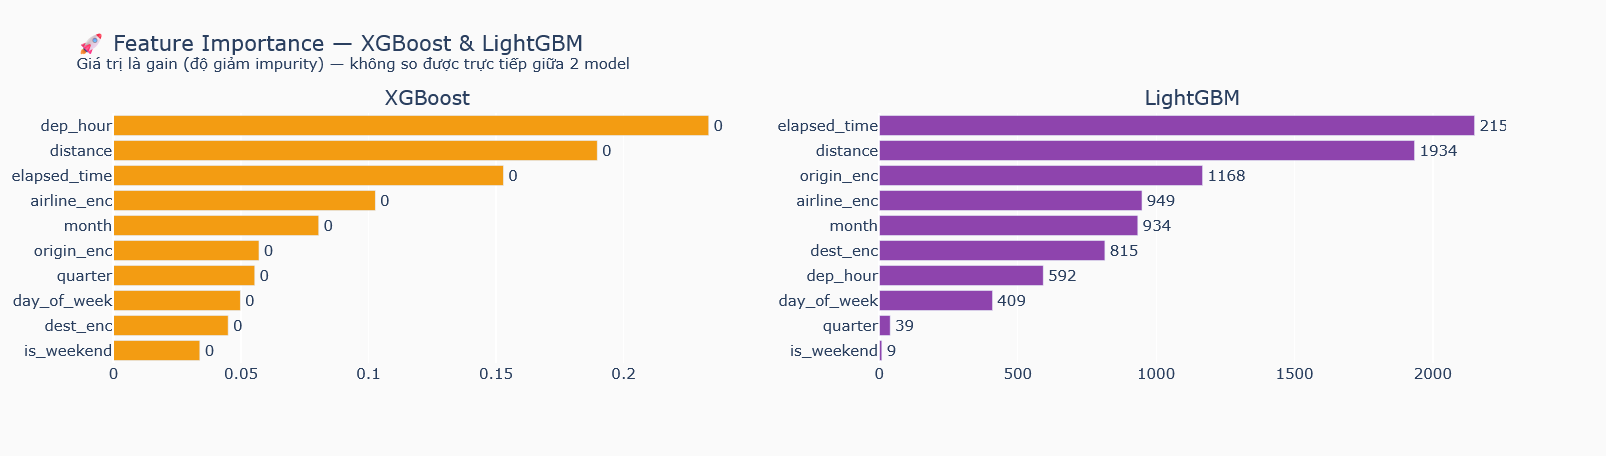
\includegraphics[width=0.75\textwidth]{img/feature_importance.png}
%     \caption{Feature Importance của mô hình LightGBM}
%     \label{fig:feature_importance}
% \end{figure}

\subsubsection{Phân tích tại sao Gradient Boosting thắng}

Các lý do Gradient Boosting (XGBoost/LightGBM) đạt hiệu suất tốt nhất:

\begin{enumerate}
    \item \textbf{Mô hình hóa phi tuyến phức tạp:} Quan hệ giữa delay và các đặc trưng (giờ bay,
          hãng bay, sân bay) không tuyến tính --- Logistic Regression không bắt được điều này.

    \item \textbf{Xử lý interaction features tự nhiên:} GBDT tự tạo các điều kiện kết hợp
          (ví dụ: hãng F9 \textit{và} tháng 12 \textit{và} sân bay ORD) mà không cần feature engineering tay.

    \item \textbf{Khả năng chống overfitting tốt hơn Random Forest:}
          Boosting sequential correction cho phép cây nhỏ (shallow) kết hợp với nhau hiệu quả,
          trong khi Random Forest cần cây sâu hơn để đạt độ chính xác tương đương.

    \item \textbf{Xử lý mất cân bằng lớp hiệu quả:}
          \texttt{scale\_pos\_weight} của XGBoost và \texttt{is\_unbalance} của LightGBM
          được thiết kế đặc biệt cho bài toán imbalanced classification.

    \item \textbf{LightGBM nhanh nhất trong nhóm:} Leaf-wise growth + GOSS sampling
          giúp LightGBM huấn luyện nhanh hơn XGBoost \textasciitilde{}2--5 lần với AUC tương đương.
\end{enumerate}

% ------------------------------------------------------------
\subsection{Thảo luận}

\subsubsection{Giải quyết được vấn đề gì?}

So sánh với mục tiêu ban đầu:
\begin{itemize}
    \item[$\checkmark$] \textbf{Data Warehouse:} Đã xây dựng thành công, lưu trữ toàn bộ 5,8M chuyến bay
          trong SQLite với Star Schema, hỗ trợ truy vấn OLAP linh hoạt.
    \item[$\checkmark$] \textbf{Dashboard OLAP:} Giao diện 2 cấp cung cấp insight về nguyên nhân,
          thời điểm và tác nhân delay, thay thế hoàn toàn phân tích thủ công.
    \item[$\checkmark$] \textbf{Dự báo delay:} Mô hình đạt AUC $\approx$ 0,73 --- tốt hơn baseline
          ngẫu nhiên (0,5) một cách đáng kể, có thể triển khai trong hệ thống cảnh báo sớm.
\end{itemize}

\subsubsection{Những trường hợp model còn sai và tại sao}

Mô hình có xu hướng dự đoán sai trong các trường hợp:
\begin{itemize}
    \item \textbf{Delay đột xuất do thời tiết cực đoan:} Bão tuyết bất ngờ, mưa đá không dự báo được
          từ dữ liệu lịch sử --- model không có feature thời tiết thực tế.
    \item \textbf{Chuyến bay đầu tiên trong ngày:} \texttt{DEPARTURE\_DELAY} = 0 nhưng thực tế delay
          do lý do vận hành nội bộ của hãng (thiếu phi hành đoàn, bảo trì kỹ thuật đột xuất).
    \item \textbf{Sân bay và hãng ít dữ liệu:} Một số sân bay nhỏ/hãng nhỏ có ít mẫu huấn luyện,
          dẫn đến encoding không đại diện.
    \item \textbf{Ngày lễ đặc biệt:} Thanksgiving, Giáng sinh có hành vi delay đặc biệt khác với
          các ngày thường trong cùng tháng --- model chưa bắt được hiệu ứng này.
\end{itemize}
